\section{Processi organizzativi}\label{section:processi_organizzativi}
I processi organizzativi sono tutti quelli che riguardano l'organizzazione del gruppo \groupName.\\ Essi si suddividono in:
\begin{itemize}
  \item \textbf{Processo di gestione organizzativa};
  \item \textbf{Processo di formazione}.
\end{itemize}

\subsection{Gestione Organizzativa} \label{subsection:gestione_organizzativa}
\subsubsection {Scopo}
Lo scopo di questa sezione è quello di normare le modalità di coordinamento tra i vari membri del gruppo:
\begin {itemize}
\item Quantificare le spese;
\item Rispettare le scadenze;
\item Quantificare i rischi.
\end{itemize}
\subsubsection{Aspettative}
Le aspettative in questa fase sono le seguenti:
\begin {itemize}
\item Ottenere un'organizzazione ragionevole ed efficace tra i membri del gruppo;
\item Adottare un buon \textit{way of working};
\item Riuscire a controllare le spese;
\item Ottenere un'equa distribuzione dei ruoli, riuscendo ad avere una rotazione efficace.
\end {itemize}
\subsubsection{Descrizione}
Le attività di gestione sono:
\begin {itemize}
\item Assegnazione dei ruoli e dei compiti;
\item Inizio e definizione dello scopo;
\item Istanziazione dei processi;
\item Pianificazione e stima di tempi, risorse e costi;
\item Esecuzione e controllo;
\item Revisione e valutazione periodica delle attività.
\end {itemize}
\subsubsection{Istanziazione del processo}
\paragraph{Ruoli di progetto}
\paragraph*{\roleProjectManager{} \textit{di progetto}}
Il suo compito consiste nel garantire lo svolgimento delle attività pianificate entro i tempi e le modalità previste dal gruppo.\\
Rappresenta il gruppo nelle comunicazioni esterne con committenti e proponenti.\\
Le sue responsabilità sono:
\begin{itemize}
  \item Gestire l'assegnazione dei compiti agli altri membri del gruppo;
  \item Organizzare il lavoro in modo da minimizzare la probabilità che si verifichino problemi;
  \item Approvare la documentazione nella fase finale del processo di verifica.
\end{itemize}

\paragraph*{\roleAdministrator{}}
È responsabile degli strumenti necessari all'ambiente di lavoro.\\
Le sue responsabilità sono:
\begin{itemize}
  \item Gestire il sistema di archiviazione e versionamento di documentazione e codice;
  \item Gestire il sistema di configurazione e versionamento del prodotto;
  \item Mantenere efficiente l'ambiente di sviluppo, fornendo strumenti adeguati ai membri del gruppo;
  \item Redigere le \docNameVersionNdP{} che l'intero gruppo deve seguire;
  \item È responsabile della redazione e attuazione di piani e procedure di gestione per la qualità.
\end{itemize}

\paragraph*{\roleAnalyst}
Il suo compito consiste nell'individuare, analizzare e documentare i servizi che il sistema deve fornire.\\
Le sue responsabilità sono:
\begin{itemize}
  \item Analizzare la complessità del problema generale e delle funzionalità da implementare;
  \item Modellare concettualmente il sistema;
  \item Individuare i requisiti del progetto e suddividerli in categorie;
  \item Redigere la \docNameVersionAdR{}.
\end{itemize}

\paragraph*{\roleDesigner}
Il suo compito consiste nel definire la struttura architetturale del sistema.\\
È responsabile delle attività di progettazione, le quali devono portare alla realizzazione di un prodotto in grado di soddisfare i requisiti individuati dagli analisti.\\
Le sue responsabilità sono:
\begin{itemize}
  \item Studiare l'architettura più adatta al prodotto da realizzare;
  \item Garantire la qualità del prodotto;
  \item Identificare l'architettura ad alto livello del sistema e l'architettura a livello di componenti del sistema.
\end{itemize}

\paragraph*{\roleProgrammer}
Il suo compito consiste nella scrittura del codice richiesto dallo svolgimento del progetto.\\
Le sue responsabilità sono:
\begin{itemize}
  \item Scrivere codice documentato, manutenibile e versionato;
  \item Rendere l'attività di verifica semplice svolgendo il proprio compito con gli strumenti e le modalità previsti da questo documento.
\end{itemize}

\paragraph*{\roleVerifier}
Il suo compito consiste nella verifica del progetto.\\
Le sue responsabilità sono:
\begin{itemize}
  \item Controllare che vengano rispettate le norme di progetto, inserite nell'omonimo documento \docNameVersionNdP{};
  \item Assicurarsi della conformità di ogni stadio del ciclo di vita\glo{} del prodotto;
  \item Segnalare eventuali anomalie riscontrate nella verifica in modo che vengano corrette tempestivamente.
\end{itemize}
\paragraph {Procedure}
Per il coordinamento e le comunicazioni durante l'intera durata del progetto il gruppo \groupName{} adotterà le seguenti procedure:
\begin{itemize}
  \item \textbf{Comunicazione interna:} coinvolge tutti i membri del gruppo;
  \item  \textbf{Comunicazione esterna:} coinvolge proponente e committenti.
\end{itemize}


\paragraph{Rotazione dei ruoli}
È prevista una rotazione dei ruoli a cadenza periodica da parte del gruppo \groupName{}.\\
L'attribuzione dei ruoli viene svolta secondo i seguenti criteri:
\begin{itemize}
  \item \textbf{Equità:} ogni membro del gruppo deve svolgere un numero di ore per ogni ruolo in maniera equa nei confronti degli altri membri;
  \item \textbf{Continuità:} i ruoli vengono fatti ruotare in concomitanza con l'inizio di un nuovo periodo, in modo da garantire che il lavoro svolto dai membri del gruppo abbia una continuità nel corso di ciascun periodo;
  \item \textbf{Assenza di conflitti:} poiché ogni membro può ricoprire più ruoli in un periodo, si cerca di assegnarli in modo che non ci sia conflitto di interesse tra essi. Vige in ogni caso la regola che un \roleProjectManagerLow{} non può approvare il proprio lavoro di verifica se ha assunto anche il ruolo di \roleVerifierLow{}, mentre un \roleVerifierLow{} non può verificare i propri testi o codice qualora abbia assunto il ruolo di \roleAnalystLow{} o \roleProgrammerLow{} nello stesso periodo.
\end{itemize}


\subsubsection{Impiego delle infrastrutture interne} \label{subsection:infrastrutture_interne}

\paragraph{Gestione delle comunicazioni}
\subparagraph{Comunicazioni interne}
Le comunicazioni interne del gruppo \groupName{} avvengono tramite i canali Discord\glo{} e Telegram\glo{}.\\
Il canale Discord\glo{} viene utilizzato principalmente per gli incontri settimanali tra i membri del gruppo, essendo uno strumento utilizzato anche in ambito aziendale, ciò favorisce uno spazio di lavoro condiviso tra i membri del gruppo.
Per comunicazioni rapide invece viene preferito il canale Telegram\glo{}.

\subparagraph{Comunicazioni esterne}
Le comunicazioni con utenti esterni al gruppo sono gestite dal \roleProjectManagerLow{} del progetto. Le modalità utilizzate sono le seguenti:
\begin {itemize}
\item Tramite e-mail (All'indirizzo \groupEmail{});
\item Tramite Google Meet\glo{} (Tramite link di invito mandato di volta in volta dal proponente);
\item Tramite Discord\glo{} (Tramite il server dell'azienda SyncLab).
\end {itemize}

\paragraph{Gestione degli incontri}
\subparagraph{Incontri interni}
Il \roleProjectManagerLow{} ha il compito di organizzare gli incontri interni utilizzando l'apposito canale di comunicazione.\\
Per ogni incontro viene redatto un \docNameVLow{} che raccoglie tutti gli argomenti trattati durante la riunione.
\paragraph {\textit{Verbali} di incontri interni}
In occasione di ogni incontro interno viene redatto un \docNameVLow{} dal segretario scelto dal \roleProjectManagerLow{}. Il contenuto della riunione deve essere riportato nel \docNameVLow{} corrispondente e approvato dal \roleProjectManagerLow{}.

\subparagraph{Incontri esterni}
Il \roleProjectManagerLow{} ha il compito di organizzare gli incontri esterni con il proponente o con il committente.\\
Un incontro esterno viene richiesto se vi è la necessità impellente di chiarimento di una problematica riscontrata da parte del gruppo.\\
In questo caso il \roleProjectManagerLow{} provvede a formalizzare una richiesta all'entità esterna (proponente o committente) tramite le mail di contatto fornite.\\
In caso di richiesta accettata, verranno comunicate ai membri del gruppo, tramite canali di comunicazione interni, le informazioni riguardanti data, ora e luogo dell'incontro.\\
Come per gli incontri interni, deve essere redatto un \docNameVLow{} che descriva gli argomenti trattati.
\paragraph {\textit{Verbali} di incontri esterni}
In occasione di ogni incontro esterno viene redatto un \docNameVLow{} da un redattore scelto dal \roleProjectManagerLow. Il contenuto della riunione deve essere riportato nel \docNameVLow{} esterno corrispondente e approvato dal \roleProjectManagerLow.

\paragraph{Gestione degli strumenti di coordinamento}
\subparagraph{Ticketing}
Per la suddivisione delle issue\glo{} viene utilizzato \textit{GitHub Projects Board}\glo{}.\\
Il \roleProjectManagerLow{} avrà il compito di creare e assegnare le varie issue\glo{} ai membri del gruppo.\\
\textit{GitHub Projects Board}\glo{} permette una buona gestione delle issue\glo{}, infatti:
\begin{itemize}
  \item Le issue\glo{} possono trovarsi in quattro stati diversi:
        \begin{itemize}
          \item \textbf{New:} sono presenti le issue\glo{} appena create che devono ancora essere assegnate;
          \item \textbf{To Do:} sono presenti le issue\glo{} assegnate e da portare a termine;
          \item \textbf{In progress:} sono presenti le issue\glo{} attualmente in esecuzione;
          \item \textbf{Done:} sono presenti le issue\glo{} portate a termine.
        \end{itemize}
  \item Ogni membro del gruppo ha la possibilità di spostare le proprie issue\glo{} nelle diverse colonne che rappresentano gli stati;
  \item Le issue\glo{} hanno una descrizione e possono ricevere commenti da parte degli altri componenti del gruppo;
  \item All'interno di una issue\glo{} possono essere presenti dei task sotto forma di checklist nella sezione commenti.
\end{itemize}
Ogni membro del gruppo ha il dovere di tenere aggiornate le sue attività e deve rispettare le scadenze delle varie issue\glo{}.
Se si completa un task bisogna spuntarlo come completato all'interno dell'issue\glo{}.\\
Inoltre è possibile creare delle milestone\glo{} a cui assegnare le issue\glo{}, permettendo così di stabilire un punto di
riferimento sulla linea temporale entro il quale è previsto il completamento di tali issue\glo{}.

\paragraph{Gestione degli strumenti di versionamento}
\subparagraph{Repository}
Per il versionamento dei file è stata scelta la piattaforma GitHub\glo{}. L'\roleAdministratorLow{} ha creato il repository\glo{} e ha aggiunto
come collaboratori tutti i membri del gruppo \groupName{}.

\subparagraph{Tipi di file e \textit{.gitignore}}
Nelle cartelle che contengono i documenti, sono presenti solo i file \textit{.tex} e \textit{.png}.\\
Nel file \textit{.gitignore} sono state aggiunte tutte le estensione che devono essere ignorate da un commit, al fine di evitare la presenza di file indesiderati
o non rilevanti che devono quindi non essere versionati.
\subparagraph {Gestione dei rischi}
Il \roleProjectManagerLow{} ha il compito di individuare i rischi e renderli noti. Tale attività verrà svolta nel \docNamePdPLow{} e contiene i seguenti punti:
\begin{figure}[htbp]
\centering
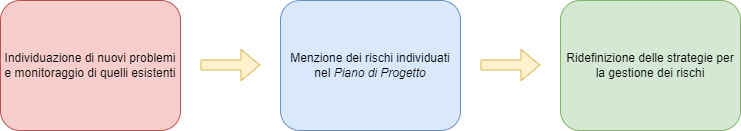
\includegraphics[scale =0.65]{../template/images/NdP/GestioneRischi.png}
\caption{Attività di gestione dei rischi}
\end {figure}

\subparagraph {Codifica dei rischi}
I rischi sono codificati nella seguente maniera: \\
\begin{center}
  \textbf{\Large{R[Tipo][ID Numerico]}}
\end{center}
dove:
\begin{itemize}[label={}]
  \item \textbf{R}: Sta per rischio;
  \item \textbf{Tipo}: Rappresenta la tipologia del rischio e può assumere uno dei seguenti valori letterali:
        \begin{table}[H]
          \centering
          \renewcommand{\arraystretch}{1.8}
          \rowcolors{2}{green!100!black!40}{green!100!black!30}
          \begin{tabular}{c|c}
            \rowcolor[HTML]{125E28}
            \multicolumn{1}{c}{\color[HTML]{FFFFFF}\textbf{Sigla}}
              & \multicolumn{1}{c}{\color[HTML]{FFFFFF}\textbf{Descrizione}} \\
            \hline
            T & Tecnologico                                                  \\
            R & Requisito                                                    \\
            O & Organizzativo                                                \\
            I & Interno                                                      \\
          \end{tabular}
          \caption{Sigle utilizzate per la codifica dei rischi}
        \end{table}
  \item \textbf{ID numerico}: È un id crescente che parte da 1 e viene incrementato di 1 per ciascun rischio.\\
\end{itemize}
La codifica di ciascun rischio è univoca. Non possono esserci due rischi dello stesso tipo con lo stesso ID numerico.

\subsubsection{Metriche}
Questo processo non fa uso di metriche particolari.
\subsubsection{Strumenti}
Gli strumenti utilizzati in questa fase sono i seguenti:
\begin{itemize}
  \item \textbf{Discord:} utilizzato per le comunicazioni interne tra i membri del gruppo e per le riunioni con il proponente;
  \begin{center}
    \url{https://discord.com/}
  \end{center}  
  \item \textbf{Google Meet:} utilizzato per gli incontri con il proponente;
  \begin{center}
    \url{https://meet.google.com/}
  \end{center} 
  \item \textbf{Gmail:} utilizzato per le comunicazioni con i committenti ed il proponente;
  \begin{center}
    \url{https://www.google.com/intl/it/gmail/about/}
  \end{center} 
  \item \textbf{Telegram:} utilizzato per la comunicazione tra i membri del gruppo.
  \begin{center}
    \url{https://telegram.org/}
  \end{center} 
\end{itemize} 
\vspace{2cm}
\subsubsection{Metriche}
Questo processo non fa uso di metriche particolari.
\subsubsection{Strumenti}
Questo processo non fa uso di strumenti particolari.

\subsection{Formazione} \label{subsection: formazione}
\subsubsection {Scopo}
Lo scopo di questa sezione è quello di definire le norme riguardanti il processo di formazione dei membri del gruppo \groupName{} e quindi lo studio delle tecnologie utilizzate per produrre i documenti e costruire il prodotto richiesto.
\subsubsection {Aspettative}
Le aspettative per il processo di formazione sono:
\begin {itemize}
\item Ottenere una buona conoscenza di \LaTeX{};
\item Avere una buona familiarità con l'ambiente in cui si sviluppa il capitolato di interesse;
\item Avere una buona familiarità con i vari linguaggi di programmazione, delle librerie e dei vari strumenti necessari per la realizzazione del prodotto software assegnato dal proponente.
\end {itemize}
\subsubsection {Descrizione}
Il processo di formazione di ogni membro del gruppo \groupName{} è ritenuto fondamentale, e ha il fine di colmare le mancate conoscenze di uno o più componenti del gruppo nei vari ambiti che copre il capitolato di interesse, in modo da avere una formazione uniforme all'interno del gruppo.
\subsubsection{Istanziazione del processo}
La formazione di ogni singolo componente del gruppo avviene in maniera autonoma, tramite documentazione trovata in rete e tramite materiale fornito dal proponente e dai docenti.

\subsubsection{Metriche}
Il processo di formazione non fa uso di metriche particolari.
\subsubsection{Strumenti}
Alcuni strumenti, librerie e framework necessitano di una ampia formazione, questi sono: 

\begin{itemize}
  \item \textbf{React:} libreria JavaScript\glo{} per la creazione di interfacce utente;
  \item \textbf{\LaTeX:} linguaggio di markup per la creazione di testi;
  \item \textbf{GitHub:} Servizio di controllo di versione e hosting per progetti software;
  \item \textbf{Solidity:} Linguaggio di programmazione ad alto livello orientato agli oggetti per scrivere smart contract\glo{}.
  Viene utilizzato su varie piattaforme blockchain\glo{}, in particolare Ethereum\glo{}.

\end{itemize} 